\documentclass[10pt,a4paper]{article}
\usepackage[utf8]{inputenc}
\usepackage[T1]{fontenc}
\usepackage{graphicx}
\graphicspath{{./figures/}}

\title{MA332 Project 1}
\author{Ben Raivel}
\begin{document}
	\maketitle
	\section{Introduction}
	Newton's Method is a numerical root-finding algorithm. To find a root $ f(x_\star) = 0 $, the algorithm uses $f$, its derivative $f^\prime$, and some starting value $x_0$.

	\section{Failure to Converge}
	Depending on the function and starting value, Newton's Method may not converge.
	
	\section{Basins of Attraction}
	For a given root $ f(x_\star) = 0$, the \emph{basin of attraction} is the set of starting values $ x_0 $ for which Newton's Method will converge to $ x_\star $.
	
		\subsection{Real-Valued Functions}
		Consider the function
		$$ g(x) = (x - 1)(x + 3) $$
		
		\begin{figure}[h]
			\caption{Basins of convergence for $g(x) = (x - 1)(x + 3)$}
			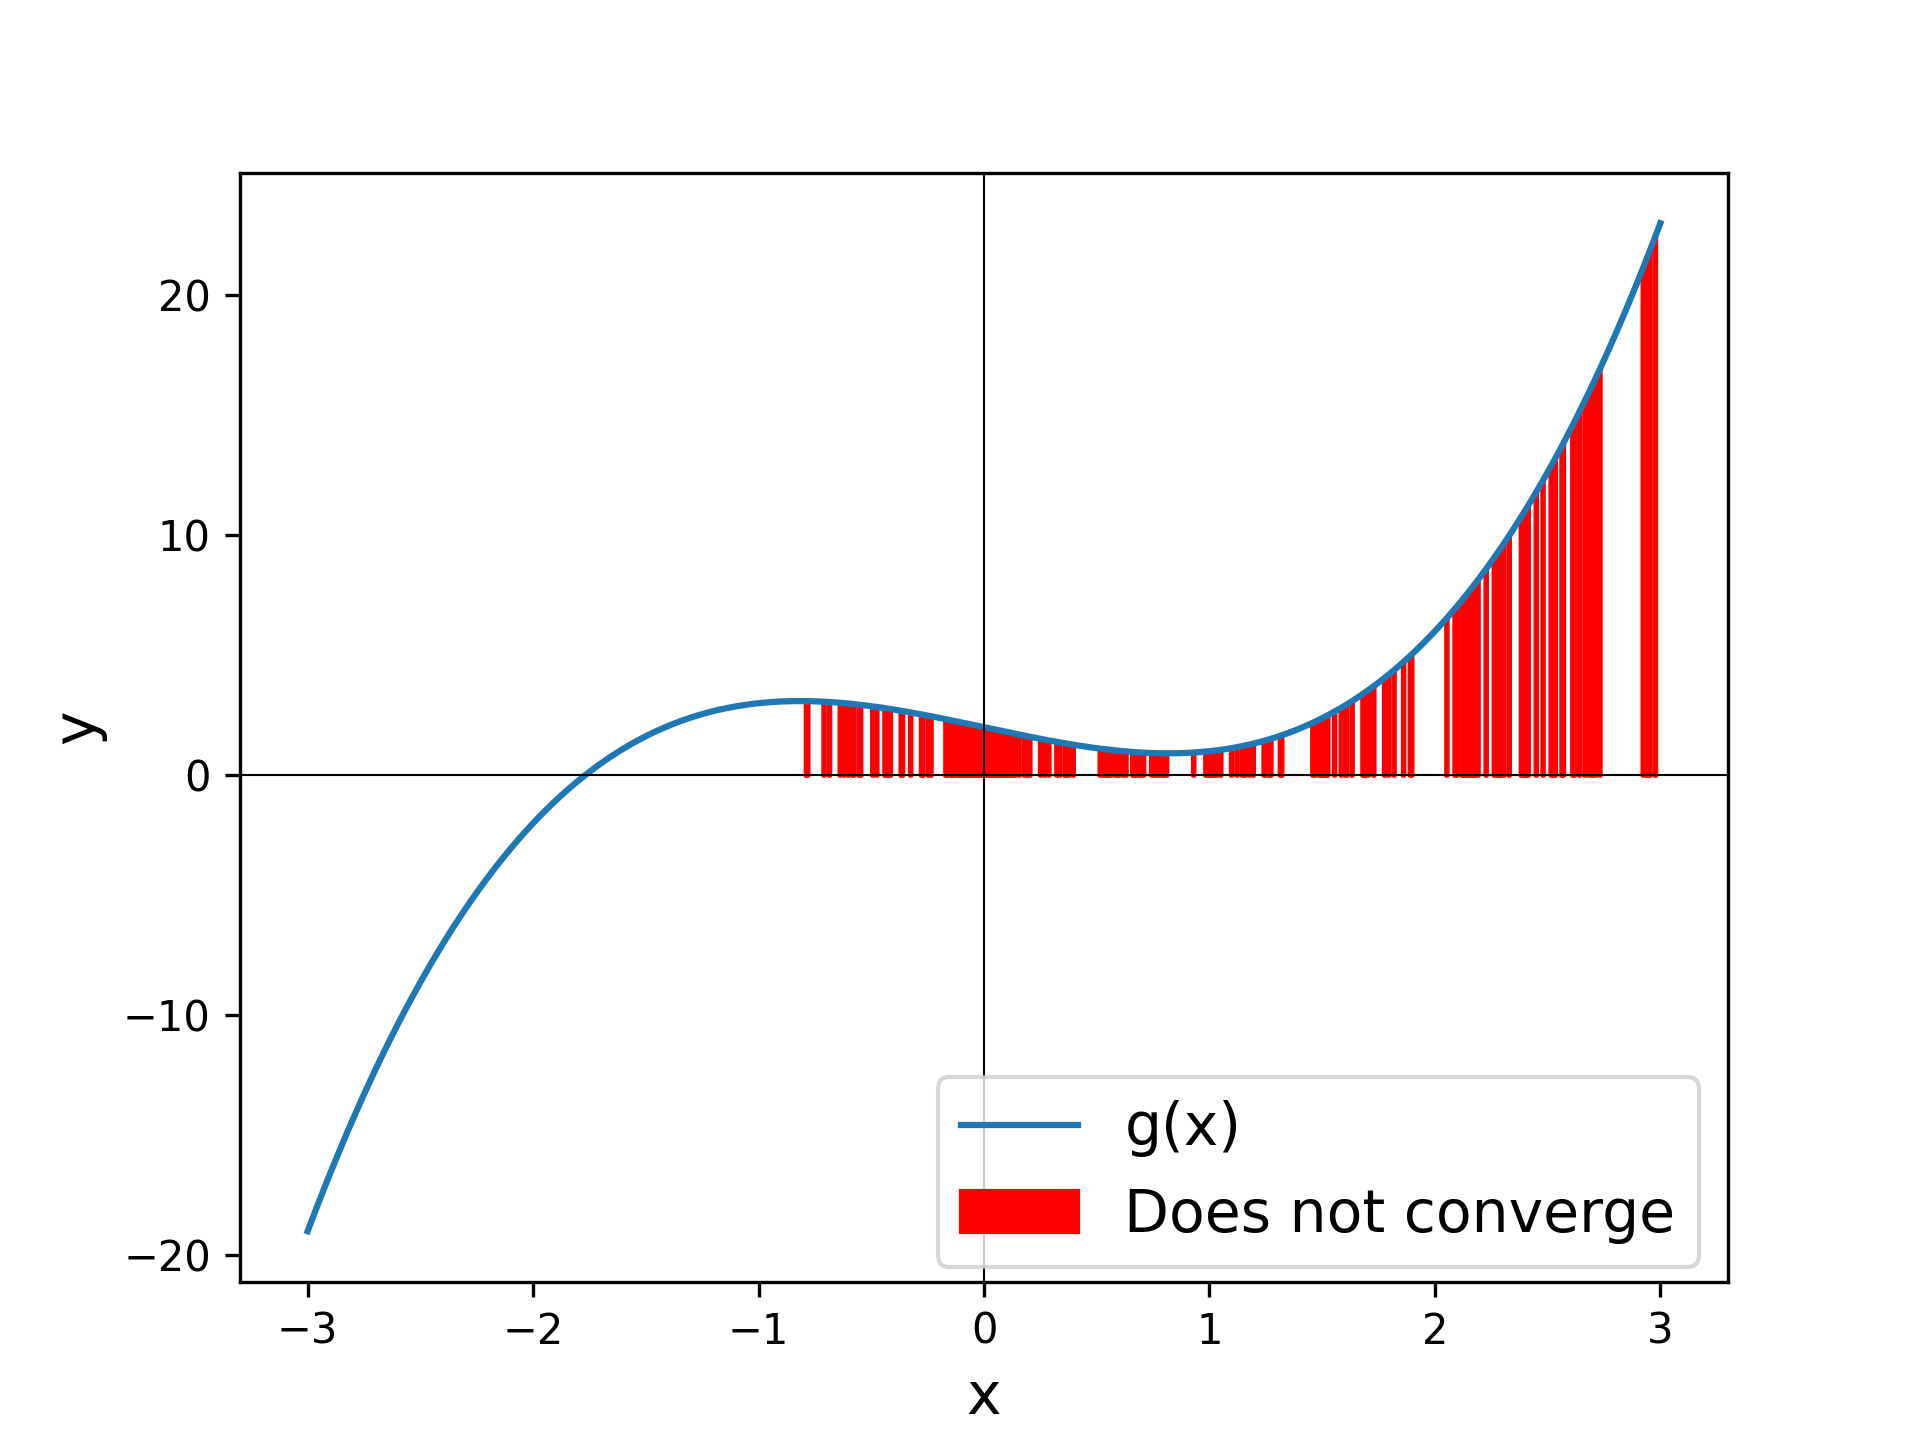
\includegraphics[scale=0.75]{figure1}
		\end{figure}
	
		\begin{figure}[h]
			\caption{Basins of convergence for $h(x) = (x - 4)(x - 1)(x + 3)$}
			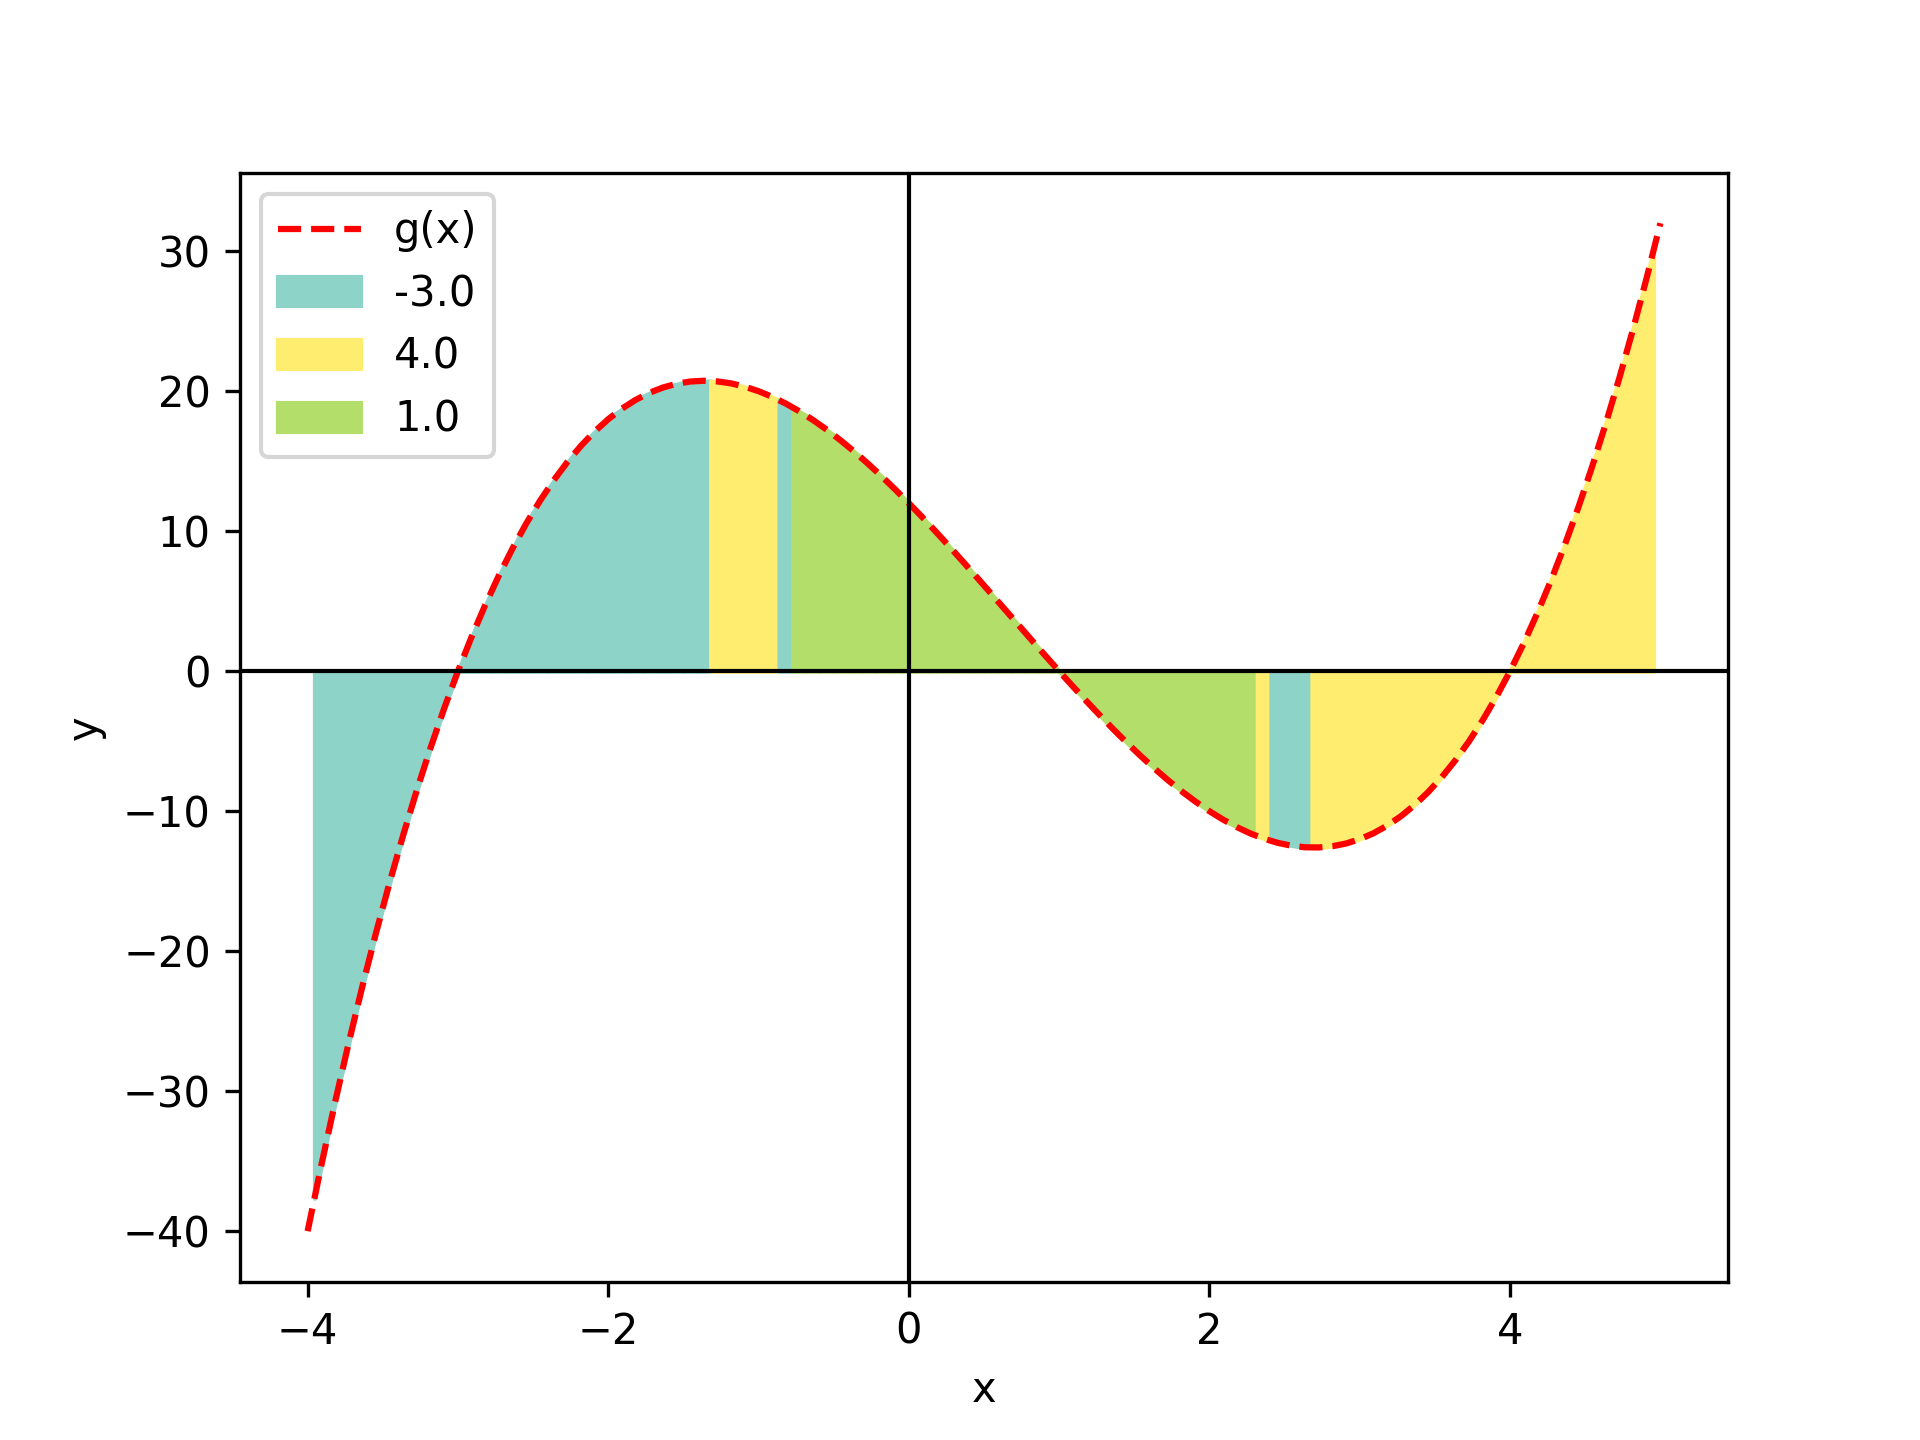
\includegraphics[scale=0.75]{figure2}
		\end{figure}
	
		\begin{figure}[h]
			\caption{Zooming in shows the fractal pattern of the basins}
			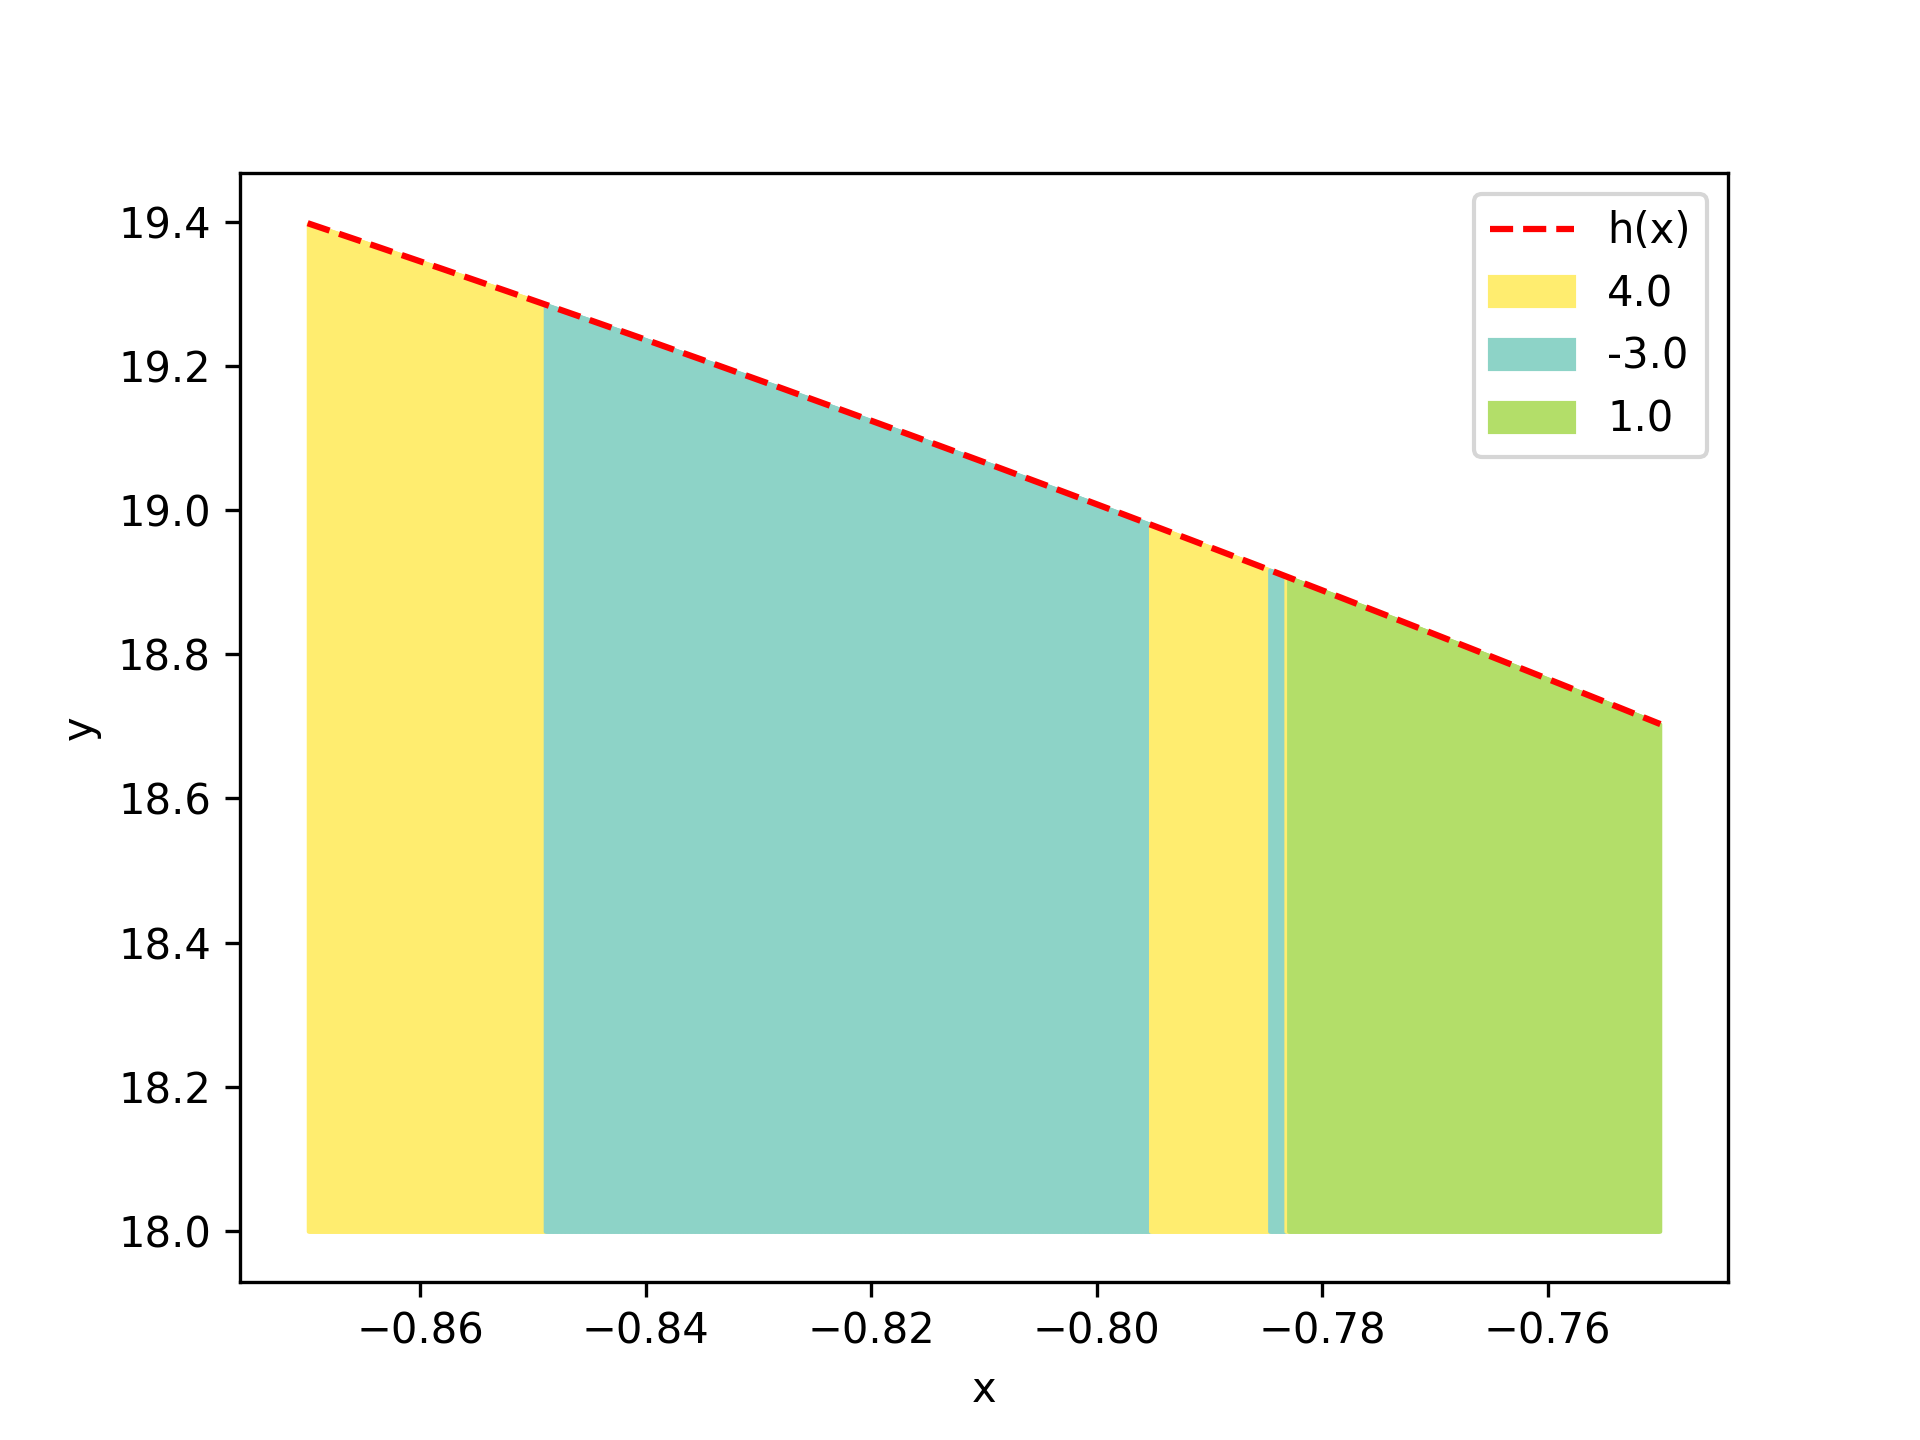
\includegraphics[scale=0.75]{figure3}
		\end{figure}

		\begin{figure}[h]
			\caption{Basins of convergence for $f(z) = z^3 - 1$ on the complex plane $a+bi$}
			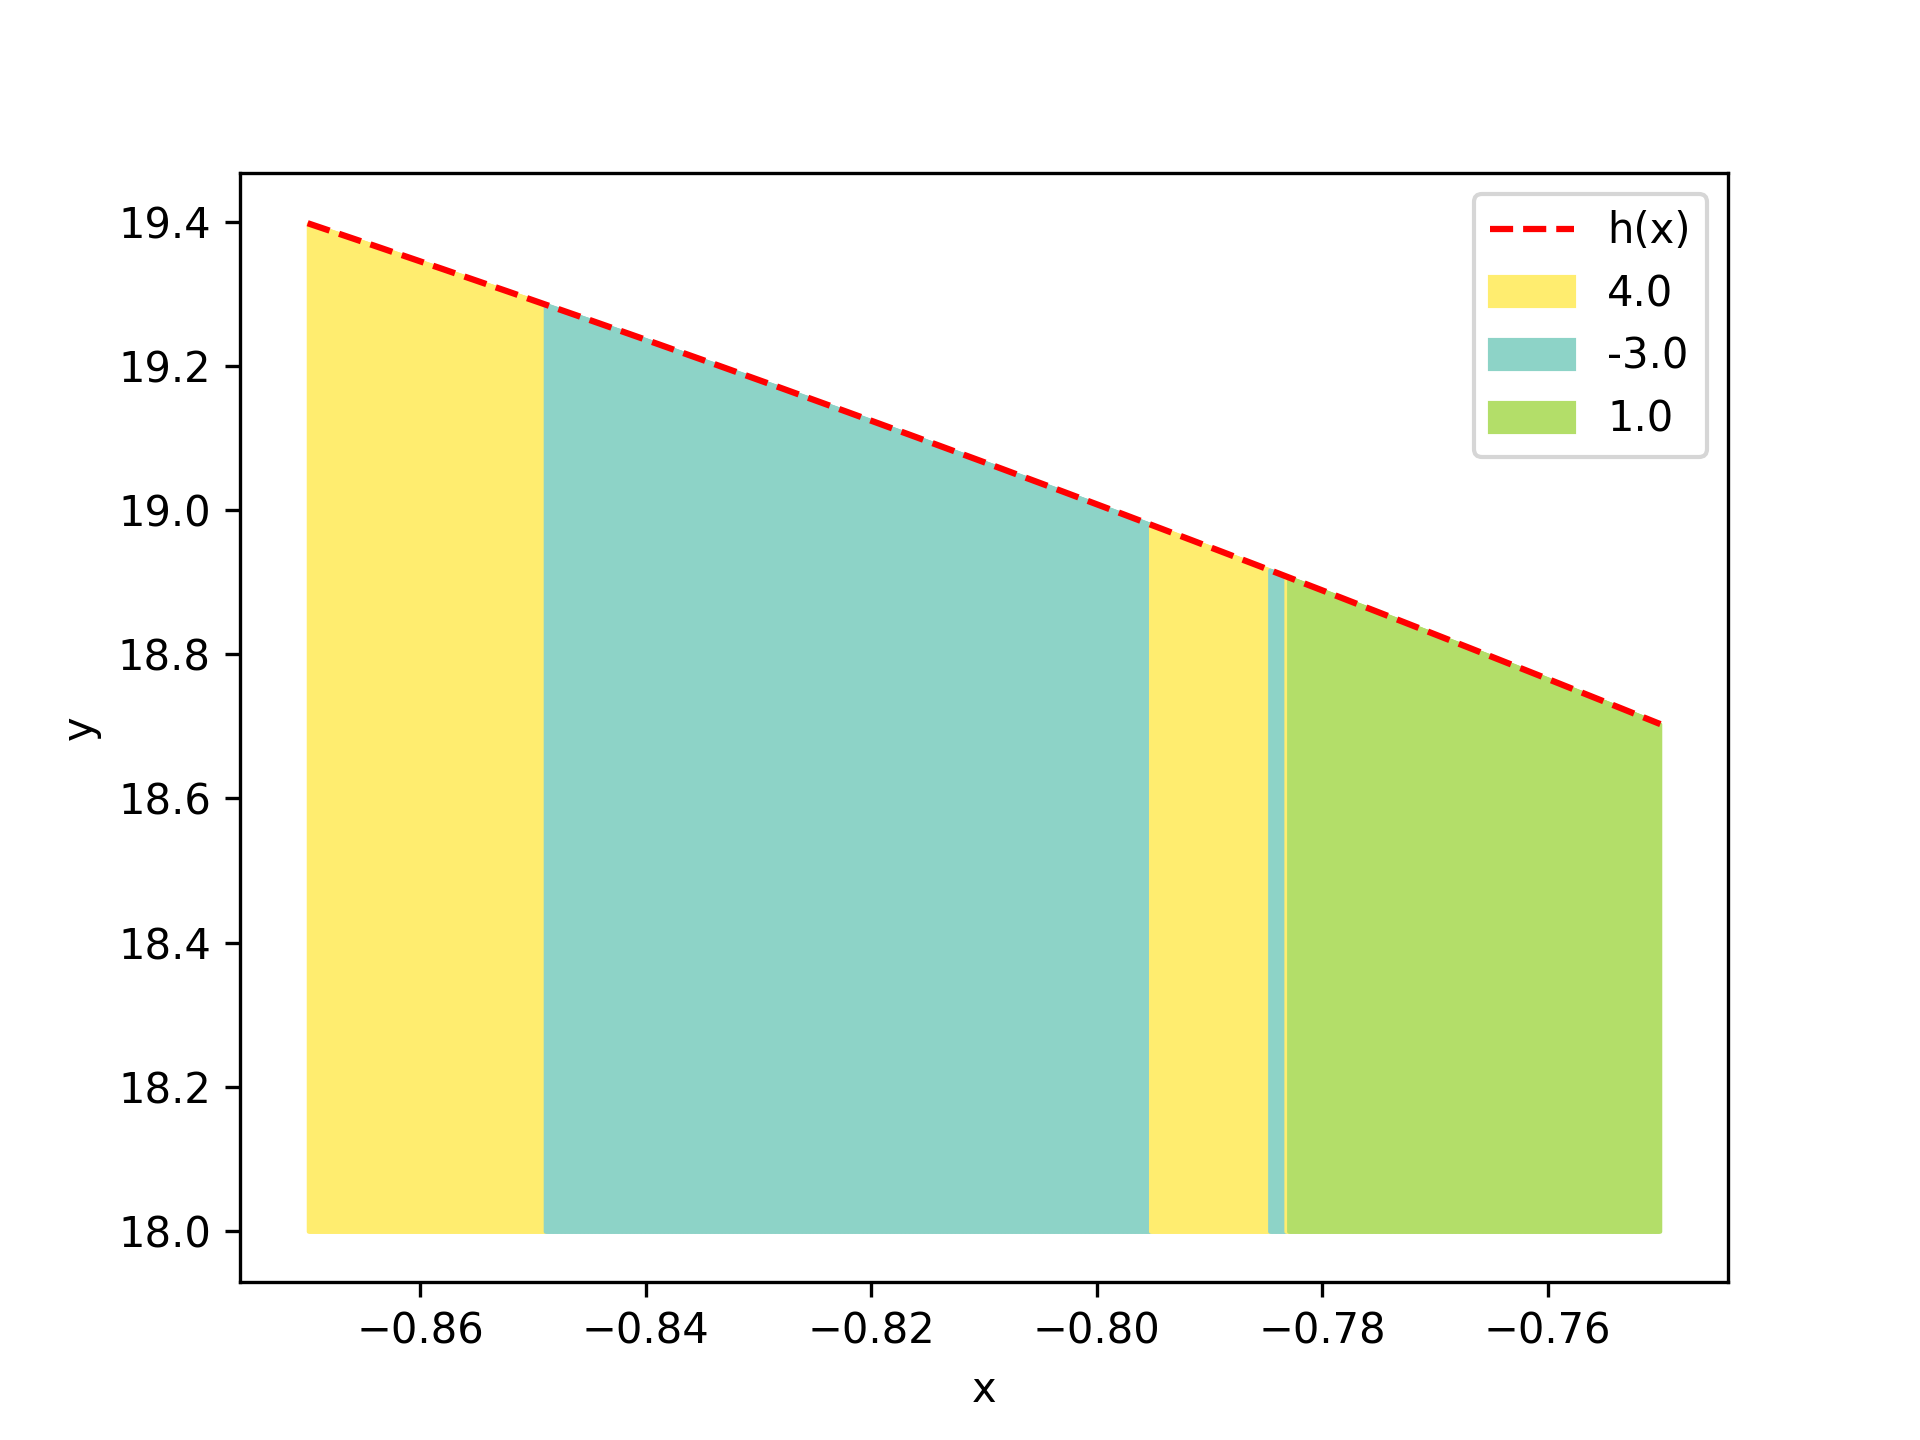
\includegraphics[scale=0.75]{figure4}
		\end{figure}
	
		\begin{figure}[h]
			\caption{Basins of convergence for $g(z) =$ on the complex plane $a+bi$}
			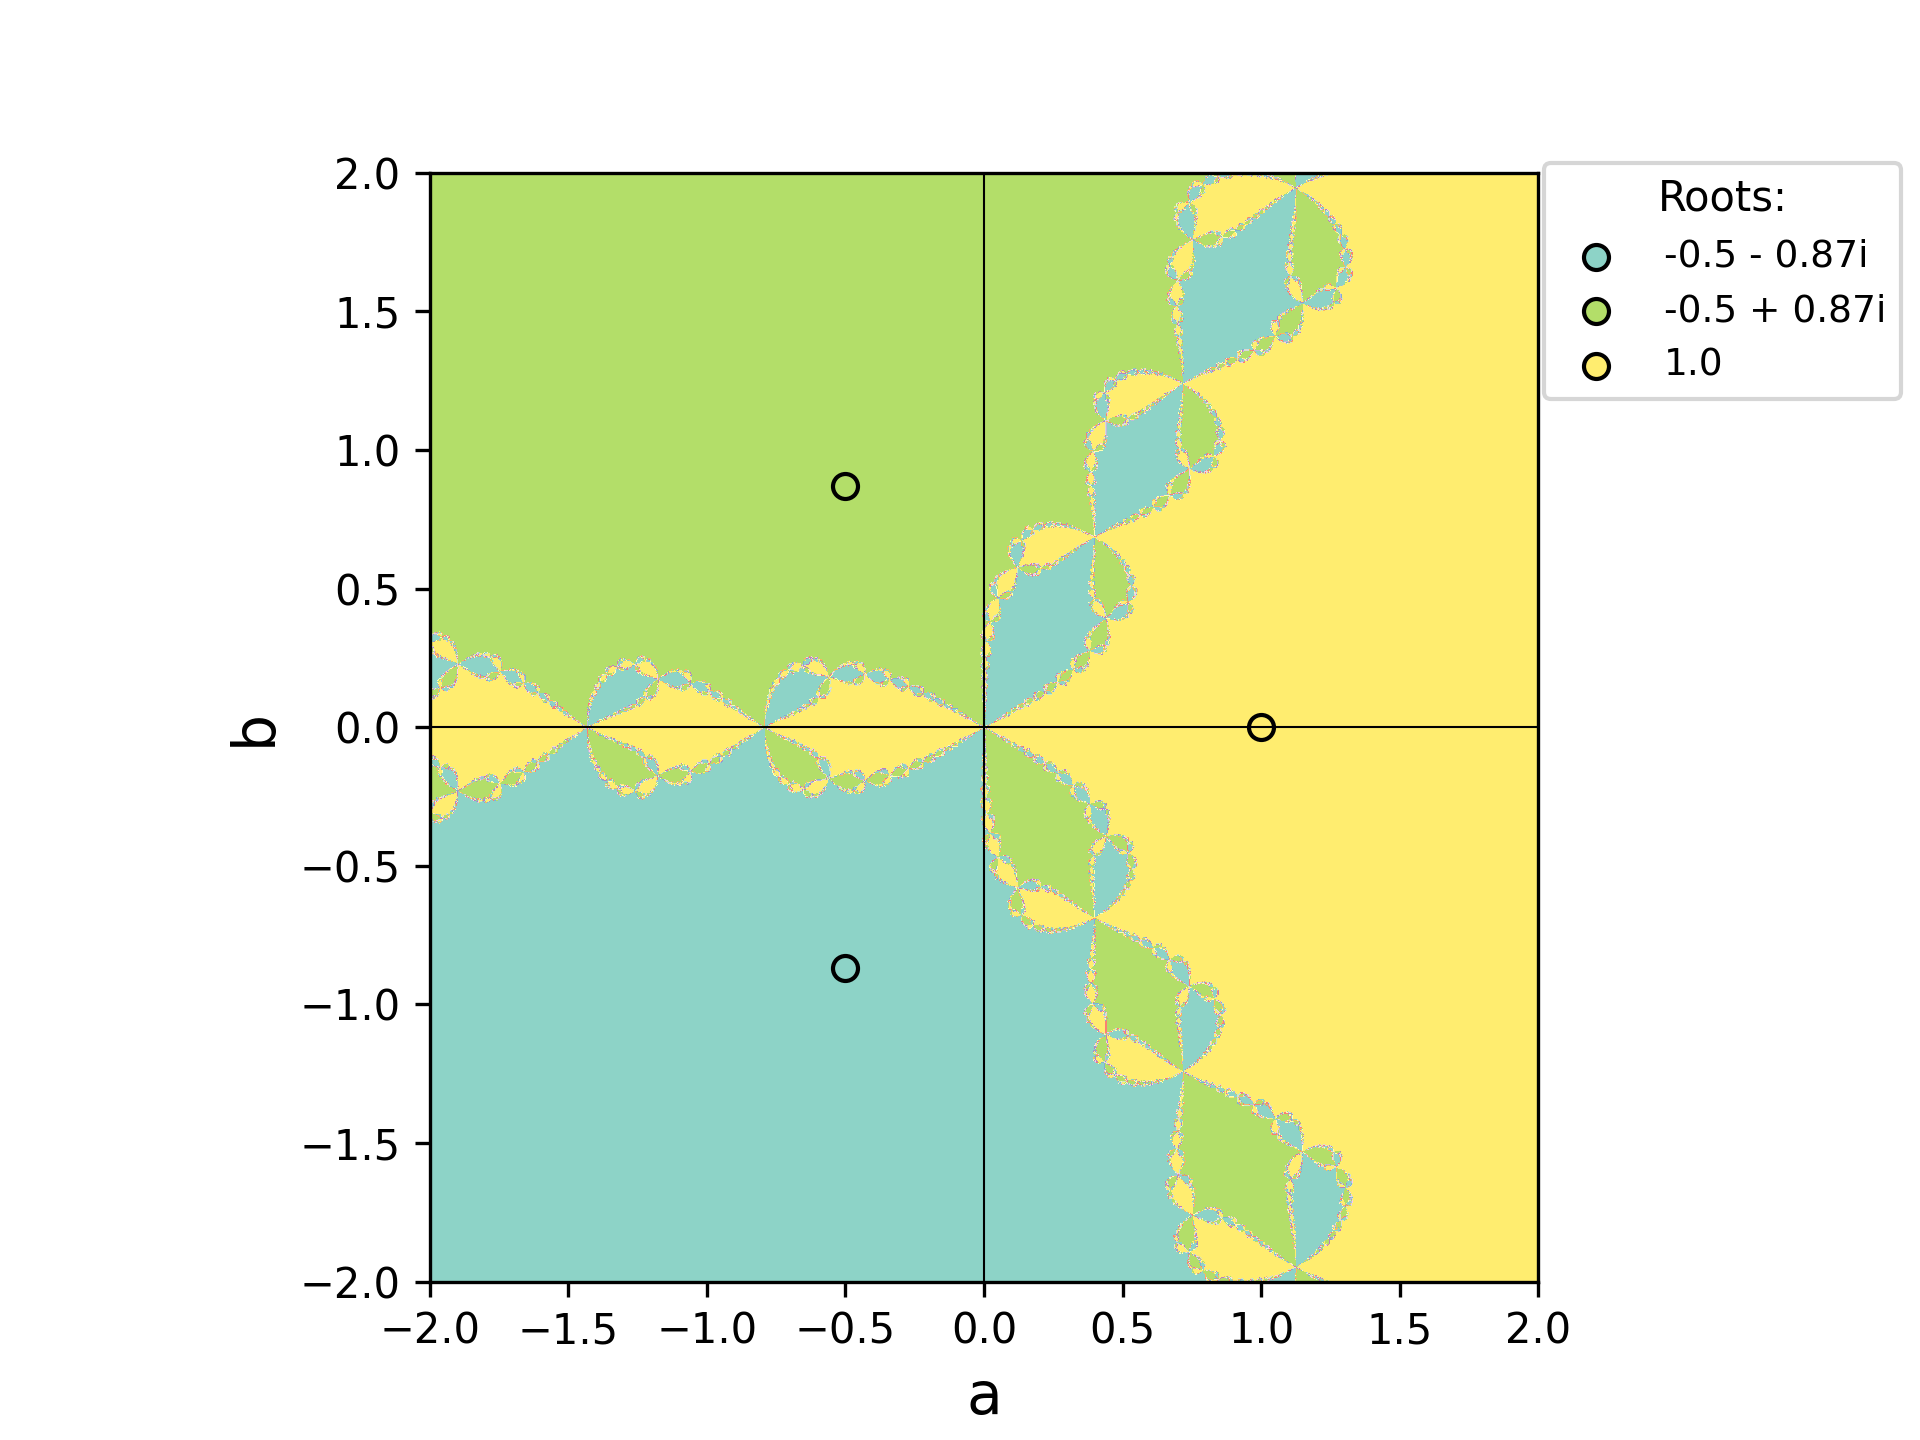
\includegraphics[scale=0.75]{figure5}
		\end{figure}
		
		\subsection{Complex-Valued Functions}
		
	\section{Discussion}
\end{document}